\documentclass[11pt,letterpaper]{article}
\usepackage{graphicx, geometry, amsmath, hyperref, url, natbib, booktabs, xcolor, listings}
\usepackage{longtable}
\usepackage{tabularx}
\usepackage{multirow}
\usepackage{array}
\usepackage{caption}
\usepackage{subcaption}
\usepackage{float}
\geometry{margin=1in}
\hypersetup{colorlinks=true, linkcolor=black, citecolor=black, urlcolor=black}

\title{Internal Research Report:\\Do Temporal Network Signals Predict\\How Scientific Concepts Spread Across Disciplines?}
\author{AI Inventor}
\date{September 2026}

\begin{document}
\maketitle
\tableofcontents
\clearpage

% ============================================================
\section{Run overview}
\label{sec:overview}

This report is the chronological record of a five-iteration research run investigating whether early structural signals in a concept's topic co-occurrence network anticipate later cross-field breadth, beyond simple measures of volume and reach. The run used the OpenAlex bulk snapshot (476{,}196{,}327 works; 2026-09-23) and identified 12{,}499 concepts, tracked 27{,}393 adoption episodes across 26 fields, and screened 53 early network indicators against a five-feature popularity baseline.

Twenty artifacts were commissioned across five iterations; sixteen completed and four failed. The run progressed through several hypothesis shifts: from citation naturalisation (iteration~1, null) to gateway-field retention (iteration~2, disconfirmed at scale) to retained-frontier relatedness (iteration~3, partial) to early ego-network openness (iterations~4--5, lead). Throughout, the headline claim narrowed and confidence decreased.

\begin{figure}[!htbp]
\centering
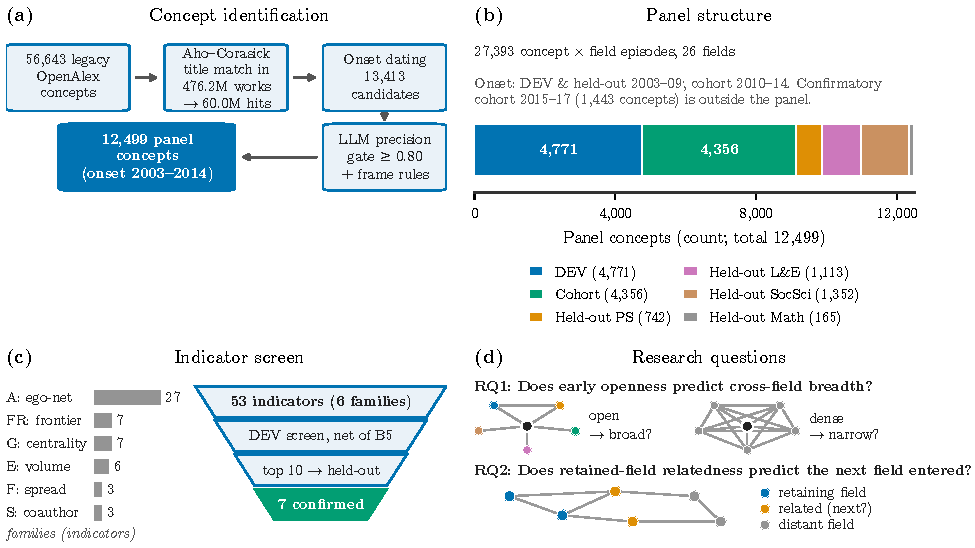
\includegraphics[width=\linewidth,height=0.85\textheight,keepaspectratio]{figures/fig_overview_v0.pdf}
\caption{Overview of the study design. (a) Concept identification: 56{,}643 legacy OpenAlex concepts are matched by title (Aho--Corasick) against a 476.2M-work OpenAlex snapshot, giving 60.0M verified matches; concepts are onset-dated ($t_0 \in$ 2003--2014), required to have early volume $\geq 30$ and to pass an LLM precision gate $\geq 0.80$, yielding an analysis panel of 12{,}499 concepts. (b) Panel structure, bar lengths proportional to concept counts: DEV (blue; CS, Eng, BGM and Med homes, onset 2003--09) 4{,}771, held-out field groups (grey; onset 2003--09) 3{,}372, and the 2010--14 onset cohort (green) 4{,}356. The expanded lower bar splits the held-out block into PHYS 742, LIFEENV 1{,}113, SOC 1{,}352 and MATHDEC 165. The panel contains 27{,}393 concept $\times$ off-home-field episodes over 26 venue fields; a separate fresh 2015--17 onset cohort of 1{,}443 concepts serves as a confirmatory frame. (c) Indicator screen for the breadth outcome (O2r\_m50). Bars are coloured by indicator family with lengths proportional to indicator counts: 53 early indicators computed over $t_0..t_0{+}2$; 48 eligible on DEV; the 10 frozen on DEV by partial Spearman correlation given the five-feature baseline B5; and the 7 confirmed on held-out units. (d) The two research questions as schematic illustrations.}
\label{fig:overview}
\end{figure}


% ============================================================
\section{Iteration 1: Wide screen of rival spread signals}
\label{sec:iter1}

\subsection{Strategy and rationale}

The run's first iteration was designed as a wide screen of five rival mechanisms for why new concepts become broadly integrated. The prior review had computed a reliability of approximately 0.32 for the initial candidate $A^*_h$ (background-adjusted lineage naturalisation gap). Rather than deepening this fragile signal, iteration~1 raced five candidates on one frozen DEV panel: (1) lineage naturalisation $A^*_h$, (2) unconnected co-author groups (candidate~S), (3) co-occurrence structural diversity~$D$, (4) frequency-free selectivity~$F$, and (5) gateway-field landing~$G$. Five artifacts were commissioned.

\subsection{Experiment~1: Does citing a concept `as your own' predict its spread?}

This artifact screened candidate $A^*_h$ on the frozen P78 dev panel (48 concepts: Biochem~13, CS~21, Engineering~3, Medicine~11).

\paragraph{Result.} $A^*_h$ does \emph{not} survive the pre-registered rule:
\begin{itemize}
\item LOGO $\Delta\rho$ for O2r over B5 $= -0.006$, 90\% concept-bootstrap CI $[-0.034, 0.017]$; $\rho_{B5} = 0.834$. FAIL.
\item Positive left-out groups: 0 of 4. FAIL.
\item Split-half reliability (Spearman--Brown) $= 0.58$. FAIL (bar 0.6).
\item $|\rho|$ with log early volume / early growth $= 0.14 / 0.18$. PASS.
\end{itemize}

\paragraph{Background homophily finding (M1).} Among 48 concepts, 100\% have a positive background log-odds ratio: every field's citing papers preferentially cite their own field above chance. $R^2$ of the raw concept-lineage log-odds ratio on the background log-odds ratio is 0.66 (90\% CI [0.39, 0.83]). Two-thirds of between-concept variance in raw lineage autonomy is general disciplinary homophily, not concept-specific integration.

\paragraph{Variance decomposition.} REML: $\tau_c = 0.29$, $\tau_{cj} = 0.65$. PyMC NUTS check passes (Spearman 0.9996 with REML).

\paragraph{Data deviation.} The shared OpenAlex credit pool ran dry (139 own credits spent). Yearly counts came from OpenAlex S0; field labels, citation lineage and background references came from free Semantic Scholar data.

\begin{table}[!htbp]
\centering
\caption{Experiment~1 screen result: candidate $A^*_h$ clause-by-clause (iteration~1, gen\_art\_experiment\_1).}
\label{tab:exp1_screen}
\small
\begin{tabular}{p{5cm}cc}
\toprule
Clause & Value & Pass \\
\midrule
$\Delta\rho \geq 0.10$, CI low $> 0$ & $-0.006$ [$-0.034$, $0.017$] & No \\
$\geq 3/4$ groups positive & 0 of 4 & No \\
Split-half $r_{SB} \geq 0.6$ & 0.583 & No \\
$|\rho|$ with vol/growth $\leq 0.6$ & 0.14 / 0.18 & Yes \\
\bottomrule
\end{tabular}
\end{table}

\subsection{Experiment~3: Do diverse topic ties predict concept spread?}

This artifact screened two co-occurrence emergence indicators ($D_{\mathrm{ratio}}$ and $F_{\mathrm{res}}$) on 47 DEV concepts under shared protocol S0.

\paragraph{Result.} Neither candidate survives:
\begin{itemize}
\item $D_{\mathrm{ratio}}$: $\Delta\rho = +0.006$, CI90 $[-0.092, 0.135]$, 3/4 groups positive, $r_{SB} = 0.83$.
\item $F_{\mathrm{res}}$: $\Delta\rho = -0.060$, CI90 $[-0.158, 0.014]$, 1/4 groups positive, $r_{SB} = 0.44$.
\end{itemize}

\paragraph{Exploratory partial association.} The out-of-group partial $\rho$ of $D_{\mathrm{ratio}}$ given B5 was 0.335 [0.02, 0.65], permutation $p = 0.037$; $\Delta\rho$ is near its ceiling because B5 is already strong ($\rho_{B5} = 0.770$).

\paragraph{Portability.} $D_{\mathrm{ratio}}$, $D_{\mathrm{rare}}$, participation and $\mathrm{NOV_{res}}$ are associated with O2r in all 4 groups (pooled $\rho$ 0.45--0.63; within-group minima as low as 0.12 for participation in CS, 0.27 for NOV$_{\mathrm{res}}$ in CS, 0.33 for $D_{\mathrm{ratio}}$ in Eng), but are redundant under $\Delta\rho$. Degree, strength and new-edge growth are CS-only (a negative result).

\begin{table}[!htbp]
\centering
\caption{Experiment~3 screen result (iteration~1, gen\_art\_experiment\_3).}
\label{tab:exp3_screen}
\small
\begin{tabular}{lcccccc}
\toprule
Indicator & $\Delta\rho$ & CI90 & Groups+ & $r_{SB}$ & Survives \\
\midrule
$D_{\mathrm{ratio}}$ & $+0.006$ & $[-0.092, 0.135]$ & 3/4 & 0.83 & No \\
$F_{\mathrm{res}}$ & $-0.060$ & $[-0.158, 0.014]$ & 1/4 & 0.44 & No \\
\bottomrule
\end{tabular}
\end{table}

\subsection{Experiment~4: Where a concept lands early vs how broadly it spreads}

This artifact screened gateway landing $G$ on 46 DEV concepts and produced the authoritative S0 outcome tables.

\paragraph{Result.} $G$ does not survive the pre-registered rule: $\Delta\rho = +0.033$, CI90 $[-0.095, 0.168]$, positive in 2/4 groups, $r_{SB} = 0.92$. However, B5 reaches only $\rho = 0.327$ on these 34 concepts with an outcome window (per group: CS~0.10, Eng~0.86, BGM~0.65, Med~0.57), much weaker than in Experiments~1 and~3. So the ceiling argument does not apply to $G$.

\paragraph{Field-level retention lead.} Adding the adopting field's eigenvector gateway centrality raised retention AUC from 0.705 to 0.808 ($+0.103$, 95\% CI [0.034, 0.167]) on 80 episodes. This was the only lead from iteration~1, carried forward for testing.

\paragraph{Next-field entry.} Relatedness density AUC 0.61 beats the permutation null ($p = 0.023$) but loses to log field size (0.74).

\begin{table}[!htbp]
\centering
\caption{Experiment~4 screen result (iteration~1, gen\_art\_experiment\_4).}
\label{tab:exp4_screen}
\small
\begin{tabular}{lcccc}
\toprule
Indicator & $\Delta\rho$ (O2r) & CI90 & Groups+ & $r_{SB}$ \\
\midrule
$G$ (gateway landing) & $+0.033$ & $[-0.095, 0.168]$ & 2/4 & 0.92 \\
\bottomrule
\end{tabular}
\end{table}

\subsection{Failed artifacts}

Two iteration-1 artifacts failed:
\begin{itemize}
\item \textbf{gen\_art\_dataset\_1} (Sealed test set of new science concepts): stalled, never completed. The outcome-blind held-out frame was not built.
\item \textbf{gen\_art\_experiment\_2} (Do independent author groups predict spread?): candidate~S, testing Cheng et al.'s co-author independent-groups hypothesis, stalled and never ran. Candidate~S was therefore untested, not refuted, at this stage.
\end{itemize}

\subsection{Iteration~1 dead ends}

\begin{enumerate}
\item $A^*_h$ naturalisation gap: null ($\Delta\rho = -0.006$, 0/4 groups).
\item Co-occurrence diversity $D_{\mathrm{ratio}}$: null ($\Delta\rho = +0.006$), though the exploratory partial association is marginal.
\item Frequency-free selectivity $F_{\mathrm{res}}$: null ($\Delta\rho = -0.060$), unreliable ($r_{SB} = 0.44$).
\item Gateway landing $G$: null on concept-level breadth ($\Delta\rho = +0.033$), but the field-level retention lead (+0.103) is carried forward.
\item CS-only co-occurrence growth indicators (degree, strength, new-edge-rate): do not generalise beyond CS.
\end{enumerate}

\subsection{Iteration~1 review and hypothesis update}

The review scored 3 (blocking) with soundness 1, citing conclusions that contradicted the run's own evidence (e.g., a ceiling argument applied to Exp4 where $\rho_{B5} = 0.327$). The hypothesis update moved from $A^*_h$ to the field-level gateway-retention lead ($\Delta$AUC $+0.103$, dev only, 80 episodes), with the unit of analysis shifting to concept $\times$ field adoption episodes. The move was \textbf{deepen}: build the held-out frame from the free snapshot, test gateway retention at scale, and address RQ2 (next-field entry and trajectories).


% ============================================================
\section{Iteration 2: Do hub fields keep new concepts?}
\label{sec:iter2}

\subsection{Strategy and rationale}

Iteration~2 moved the budget from more metrics to more samples. Five artifacts were commissioned: (1) Experiment~5, a decisive held-out test of gateway retention on a zero-credit 12{,}499-concept panel; (2) Experiment~6, testing next-field entry and trajectories; (3) Evaluation~1, stress-testing the iteration-1 lead; (4) Dataset~2, external-recognition ground truth; (5) Research~1, related-work positioning.

\subsection{Experiment~5: Held-out test of gateway-field retention}

One zero-credit scan of the full OpenAlex S3 snapshot built the authoritative S1 frame: 12{,}499 concepts (DEV 4{,}771; held-out PHYS 742, LIFEENV 1{,}113, SOC 1{,}352, MATHDEC 165; cohort 4{,}356) and 27{,}393 episodes.

\paragraph{H1 result: DISCONFIRMED.} Held-out $\Delta$AUC $= -0.00001$ [$-0.0006$, $+0.0003$]; DerSimonian--Laird pooled $-0.00004$ ($I^2 = 0$). Minimum detectable $\Delta$AUC: 0.004.

\paragraph{Baseline ladder.} Gateway's DEV signal ($+0.0019$ over the iteration-1 base) vanishes once the leave-concept-out field propensity $P_j(-c)$ is added, and reverses on held-out ($-0.0016$). Gateway alone has AUC 0.605 on DEV vs 0.506 on held-out (0.41 in SOC). Gateway is a domain-specific proxy for ``fields that keep things,'' not a position-dependent causal factor.

\paragraph{H3 (concept-level gateway landing).} Held-out partial $\rho$: $G = 0.030$, $G_A = 0.026$, $G_{\mathrm{btw}} = 0.046$ (Holm $p = 0.0045$); DL-pooled $G = 0.068$ [0.029, 0.107]. The concept-bootstrap CI of pooled $G$ is [$-0.006$, 0.065], which includes zero. DEV-to-held-out shrinkage is from 0.138 to 0.030.

\begin{table}[!htbp]
\centering
\caption{Experiment~5 panel composition (iteration~2, gen\_art\_experiment\_5).}
\label{tab:exp5_panel}
\small
\begin{tabular}{lrr}
\toprule
Split & Concepts & Episodes \\
\midrule
DEV (CS/Eng/BGM/Med, onset 2003--09) & 4{,}771 & 9{,}079 \\
Cohort (onset 2010--14, all fields) & 4{,}356 & 9{,}799 \\
Held-out Physical Sciences & 742 & 1{,}662 \\
Held-out Life \& Environment & 1{,}113 & 3{,}099 \\
Held-out Social Sciences & 1{,}352 & 3{,}320 \\
Held-out Math \& Decision Sci. & 165 & 434 \\
\midrule
\textbf{Total} & \textbf{12{,}499} & \textbf{27{,}393} \\
\bottomrule
\end{tabular}
\end{table}

\subsection{Experiment~6: Where new scientific concepts spread next}

Tested the retained-frontier claim on 653 newborn concepts (1{,}865 episodes): does relatedness to fields currently retaining a concept predict which field it enters next?

\paragraph{H2 result: CONFIRMED by the frozen rule.} Held-out LR $= 71.7$ ($p = 2 \times 10^{-17}$), $d_0 = 0.302$ [0.240, 0.369]; DL pooled $d_0 = 0.284$ [0.216, 0.352], $I^2 = 0$. Label-permutation $p = 0.001$, rewired-backbone $p = 0.015$.

\paragraph{Gateway weighting adds nothing.} M3 vs M1 permutation $p = 0.17$ (held-out), 0.31 (DEV).

\paragraph{Trajectories.} DTW $k$-medoids $k = 2$ stable (bootstrap ARI 1.0): volume-matched ``integrating'' vs ``localised'' classes (held-out independent recluster ARI 0.54; localised class dominated by Medicine homes). The HMM (6 states) gives HMM-vs-DTW ARI of 0.094, a robustness failure of the ``two stable classes'' claim.

\paragraph{Ordering.} First retained gateway field precedes entropy take-off in 66\% of broad concepts (sign $p = 0.003$) vs 57\% for peripheral fields (McNemar $p = 0.09$). However, the lead-lag regression shows negative coefficients, a significant pre-trend (ev$_{-3} = -0.072$, $p = 0.0002$), and on DEV the reverse path is significant ($b = 0.232$, $p = 0.006$). The ordering result was later reclassified as MIXED.

\subsection{Evaluation~1: Stress-testing the gateway-field retention lead}

\paragraph{Result: gateway retention FAILS.} Union panel (362 de-duplicated episodes, 54 concepts): $\Delta$AUC $= +0.001$ [$-0.012$, 0.012]; DL pooled $+0.0015$ ($I^2 = 0$). The shuffled-$R$ placebo's 95th percentile (0.130) exceeds the original $+0.103$, so the iteration-1 lead cannot be certified as above chance on 80 episodes.

\paragraph{O1 label-coverage artefact.} All 8 $G$-variant O1 gains ($+0.05..+0.15$) are label-coverage artefacts: $G$ $+0.072 \to +0.002$ once label coverage is controlled.

\subsection{Dataset~2: External recognition lookup table}

Built external-recognition dates (outcome O5) for 65{,}026 OpenAlex legacy concepts from MeSH (20{,}872 concepts), English Wikipedia (6{,}540 exact), Wikidata P571/P575 (1{,}425), ACM CCS, MSC, PACS/PhySH, and curated breakthrough lists. O5 was later evaluated and found unrelated to publication outcomes: pooled $\rho$ with O2r$_{m50}$ is 0.014 [$-0.045$, 0.073]; 67\% of concepts are recognised at or before $t_0$.

\subsection{Research~1: How our results compare with related papers}

Positioning study for the Applied Network Science paper. Collected 22 citable ANS papers with relation lines. Identified comparison numbers: Guevara (2016) field-entry AUC 0.896/0.715/0.682 for individuals/organisations/countries; no published retention AUC benchmark.

\subsection{Iteration~2 dead ends}

\begin{enumerate}
\item Gateway-field retention: DISCONFIRMED at scale ($\Delta$AUC $= -0.00001$).
\item H3 concept-level gateway landing: effect about 0.03 partial $\rho$, a quarter of its DEV value; pooled CI includes zero.
\item Ordering: MIXED (negative lead-lag, pre-trend, reverse path significant on DEV).
\item Two trajectory classes: DTW $k = 2$ not reproduced by HMM (ARI 0.094); localised class dominated by Medicine.
\item $G$-variant O1 gains: label-coverage artefacts.
\item Rescue and relay: not supported on held-out data.
\end{enumerate}

\subsection{Iteration~2 review and hypothesis update}

Review scored 3 (blocking), soundness~1. The hypothesis moved from gateway centrality (closed) to the retained-frontier lead from Experiment~6 ($d_0 = +0.281$). The decisive test for iteration~3: beat the conventional RCA-thresholded Hidalgo density on an independent frame.

\begin{figure}[!htbp]
\centering
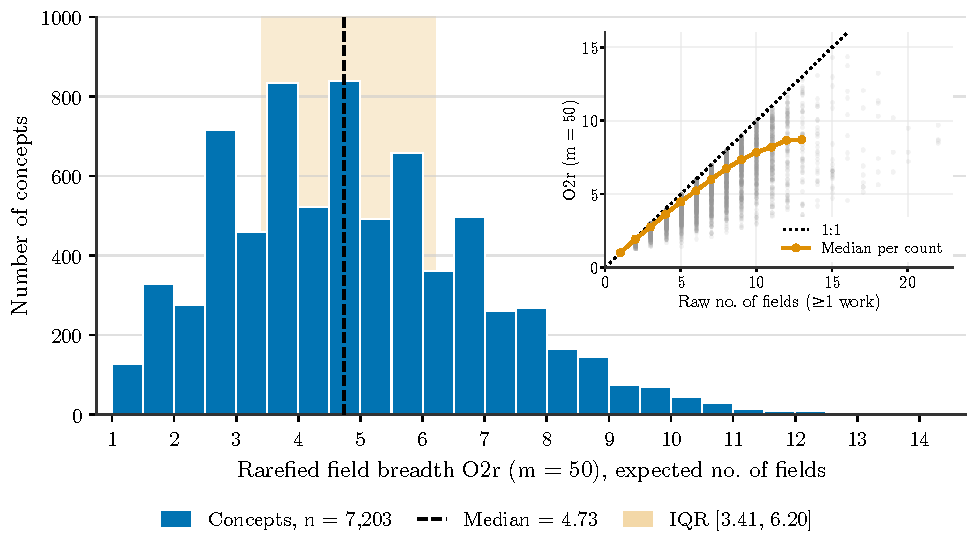
\includegraphics[width=\linewidth,height=0.85\textheight,keepaspectratio]{figures/fig_outcomes_v0.pdf}
\caption{Distribution of the primary outcome, rarefied field breadth ($O_{2r}$, $m=50$), over the 7{,}203 of 12{,}499 frame concepts that have at least 50 papers in the $t_0{+}6$..$t_0{+}8$ outcome window. (a) Histogram of $O_{2r}$; the dashed line marks the median (4.73) and the light band the IQR [3.41, 6.20]. (b) $O_{2r}$ against the raw field count.}
\label{fig:outcomes}
\end{figure}


% ============================================================
\section{Iteration 3: Decisive tests on the large panel}
\label{sec:iter3}

\subsection{Strategy and rationale}

Five artifacts were commissioned: (1) Experiment~7, the decisive retained-frontier test against the RCA-thresholded rival on an independent frame; (2) Experiment~8, the RQ1 held-out indicator screen (53 indicators, 6 families); (3) a planned RQ2 trajectories artifact (gen\_art\_experiment\_9) that failed; (4) Evaluation~2, auditing the record; (5) Research~2, prior art and venue check.

\subsection{Experiment~7: Do concepts spread from fields that keep them?}

Independent frame: 11{,}841 concepts (Exp5 minus every Exp6 concept). DEV 4{,}486 used for code; held-out scored once.

\paragraph{Result: FRONTIER = PARTIAL.} Held-out pooled $d_0 = 0.322$ [0.291, 0.355], LR(R3 vs R2) $= 325.8$ ($p < 10^{-70}$). Positive in PHYS (0.15), LIFEENV (0.40), SOC (0.30); MATHDEC (0.07, underpowered). DL over 4 groups: 0.243 [0.118, 0.368], $I^2 = 0.92$. Retained-label permutation $p = 0.001$, rewire $p = 0.004$.

\paragraph{Volume-matched contrast: null.} The pre-declared volume-matched contrast (retained vs entered-not-retained fields in the same volume cell) is $-0.028$ [$-0.105$, 0.046] on held-out (DEV: $-0.008$). Frozen verdict: FRONTIER = PARTIAL (``persistence confounded with volume'').

\paragraph{Proximity dependence.} Under Hidalgo min-conditional-probability proximity, $d_0 = -0.021$ ($p = 0.012$). The effect is backbone-specific.

\paragraph{Dose by retention age.} Held-out: 2 years $+0.098$, 3 years $+0.075$, $\geq 4$ years $+0.304$. Not monotone (held-out monotone flag: false).

\begin{table}[!htbp]
\centering
\caption{Experiment~7 field-entry results on the independent frame (iteration~3, gen\_art\_experiment\_7). Held-out pooled.}
\label{tab:exp7}
\small
\begin{tabular}{lcccc}
\toprule
Model & $d_0$ & 95\% CI & LR vs prior & Verdict \\
\midrule
R0 (home, size, density, gateway) & --- & --- & --- & --- \\
R1 (+$D_{\mathrm{rca},1y}$) & --- & --- & --- & --- \\
R2 (+$D_{\mathrm{vol}}$) & --- & --- & --- & --- \\
R3 (+$d_0$ retained) & 0.322 & [0.291, 0.355] & 325.8 & Confirmed \\
S\_strict (all rivals) & 0.304 & [0.268, 0.336] & --- & Survives \\
Volume-matched contrast & $-0.028$ & [$-0.105$, 0.046] & --- & Null \\
Min-cp proximity & $-0.021$ & --- & --- & Reverses \\
\bottomrule
\end{tabular}
\end{table}

\begin{figure}[!htbp]
\centering
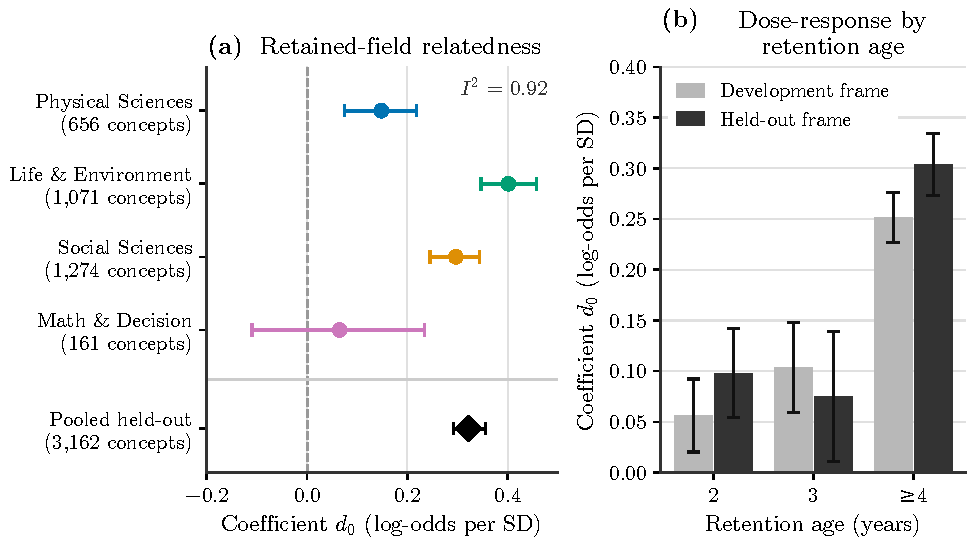
\includegraphics[width=\linewidth,height=0.85\textheight,keepaspectratio]{figures/fig_field_entry_v0.pdf}
\caption{Retained-field relatedness predicts the next field a concept enters. (a) Conditional-logit coefficient $d_0$ on the held-out groups of the independent frame. Coloured circles are per-group estimates with 95\% concept-bootstrap CIs. The black diamond is the pooled estimate, $d_0 = 0.322$ [0.291, 0.355]. (b) $d_0$ split by retention age (2, 3, $\geq$4 years).}
\label{fig:field_entry}
\end{figure}

\subsection{Experiment~8: Which early network signals travel across fields}

The RQ1 held-out deliverable: 53 indicators in 6 families (A co-occurrence ego-network 27, E popularity 6, F disciplinary spread 3, FR retained frontier 7, G gateway landing 7, S co-author 3) over $t_0..t_0+2$, plus B5 baseline. Outcomes: O1c/O1b uptake, O2r breadth, O3 transience, O4 citation growth, O5 external recognition.

\paragraph{Breadth result.} 7 of 10 frozen indicators confirmed with 6/6 unit sign agreement for O2r$_{m50}$; 8 of 10 for O2r$_{\mathrm{resid}}$.

\begin{table}[!htbp]
\centering
\caption{Held-out indicator screen: the 10 frozen indicators for rarefied breadth (O2r$_{m50}$), tested on held-out groups. DerSimonian--Laird pooled estimates with 95\% CI (iteration~3, gen\_art\_experiment\_8).}
\label{tab:exp8_screen}
\small
\begin{tabular}{llccccc}
\toprule
Indicator & Family & Pooled PSP & 95\% CI & $I^2$ & Sign & Confirmed \\
\midrule
M0\_density\_end & FR & $+0.375$ & [$+0.279$, $+0.462$] & 0.74 & 6/6 & \textbf{Yes} \\
D\_vol\_end & FR & $+0.307$ & [$+0.256$, $+0.356$] & 0.10 & 6/6 & \textbf{Yes} \\
CONTACT\_REACH & FR & $+0.211$ & [$+0.161$, $+0.261$] & 0.00 & 6/6 & \textbf{Yes} \\
$n_{\mathrm{comm}}$ (W3) & A & $+0.167$ & [$+0.063$, $+0.267$] & 0.78 & 6/6 & \textbf{Yes} \\
NOV$_{\mathrm{res}}$ & A & $+0.151$ & [$+0.044$, $+0.255$] & 0.75 & 6/6 & \textbf{Yes} \\
RETENTION\_RATIO & FR & $-0.114$ & [$-0.160$, $-0.067$] & 0.00 & 6/6 & \textbf{Yes} \\
ego\_density (W3) & A & $-0.102$ & [$-0.151$, $-0.053$] & 0.00 & 6/6 & \textbf{Yes} \\
Rao--Stirling & A & $-0.072$ & [$-0.153$, $+0.010$] & 0.44 & 5/6 & No \\
$G_{\mathrm{btw}}$ & G & $+0.056$ & [$-0.006$, $+0.118$] & 0.33 & 6/6 & No \\
log offhome vol. & F & $-0.089$ & [$-0.171$, $-0.007$] & 0.63 & 5/6 & No \\
\bottomrule
\end{tabular}
\end{table}

\begin{figure}[!htbp]
\centering
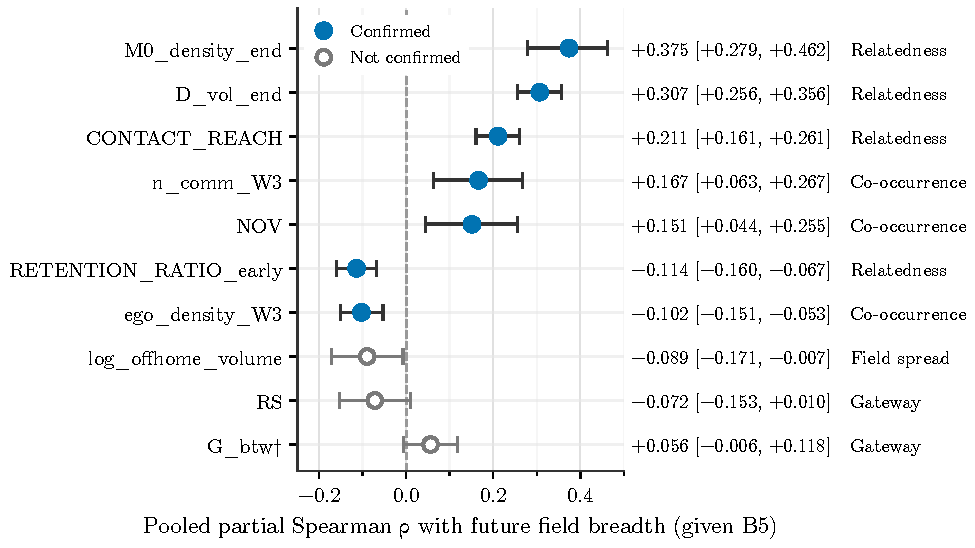
\includegraphics[width=\linewidth,height=0.85\textheight,keepaspectratio]{figures/fig_rq1_confirmed_v0.pdf}
\caption{Held-out screen of the 10 frozen indicators for rarefied cross-field breadth (O2r\_m50). Each row shows the DerSimonian--Laird pooled partial Spearman $\rho$ given B5. Filled circles are confirmed; open circles are not. Seven of the ten are confirmed across two families: retained frontier (FR) and co-occurrence topology (A).}
\label{fig:rq1_confirmed}
\end{figure}

\begin{figure}[!htbp]
\centering
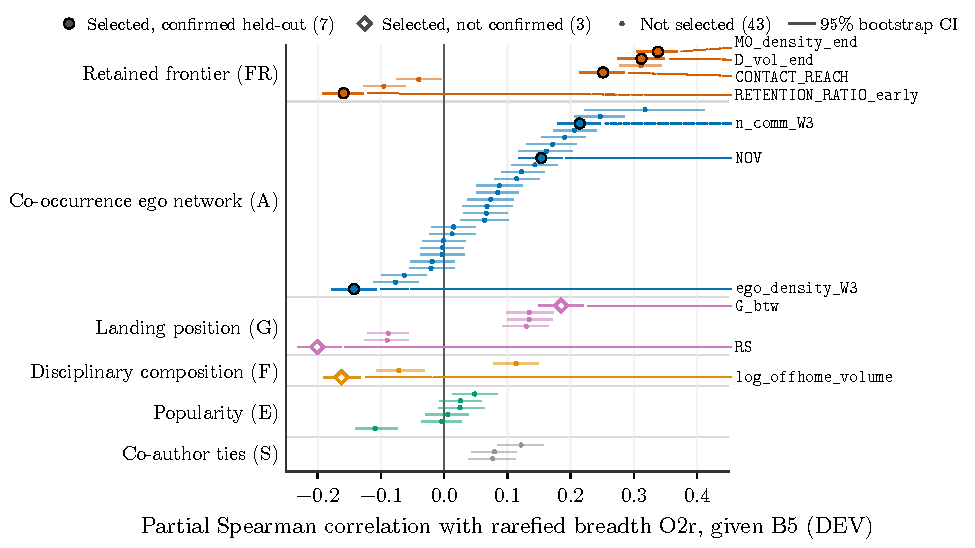
\includegraphics[width=\linewidth,height=0.85\textheight,keepaspectratio]{figures/fig_full_screen_v0.pdf}
\caption{Complete indicator screen for rarefied cross-field breadth (O2r). (a) PSP of all 53 screened indicators on the DEV fields, one row per family. Large filled circles are the 7 confirmed; large open circles are the 3 selected but not confirmed; small dots are the 43 not selected. (b) The frozen top 10 in DEV rank order with held-out pooled estimates.}
\label{fig:full_screen}
\end{figure}

\paragraph{Learned models.} ElasticNet combining all indicators adds Spearman $+0.059$ [$+0.046$, $+0.073$] over B5 on held-out; EBM adds $+0.052$ [$+0.037$, $+0.067$].

\paragraph{Pre-onset footprint caveat.} M0\_density\_end and D\_vol\_end use cumulative field history from 1995 to $t_0+2$. Part of their signal therefore predates onset.

\paragraph{Secondary outcomes.} O1c: only n\_authors\_early confirmed ($+0.161$). O4 citation growth: REL\_home $-0.114$, author\_growth $+0.065$; EBM Spearman 0.188 vs B5 0.015. O3 transience: n\_authors\_early is the only confirmed indicator; L1-logit AUC $+0.093$ over B5 at chance (0.506). O5 external recognition: no indicator or model beats B5 + onset year.

\subsection{Failed artifact: gen\_art\_experiment\_9}

The planned RQ2 trajectories artifact (contact $\times$ retention decomposition, DTW+HMM typology, sequence tests, case studies) was commissioned but never executed: the output-format validation loop failed after 5 retries. This was iteration~3's entire RQ2 artifact.

\subsection{Evaluation~2: Auditing the record before the paper}

Audited 246 claims from the record: 224 MATCH, 15 MISLABELLED, 6 MISMATCH, 1 FILE\_\allowbreak FLAG\_\allowbreak OVERRIDDEN.
Produced insert-ready corrections in 14 blocks and record tables.
Validated O5: precision 0.86, dates within 1 year 95\%, false-negative rate $\geq 0.14$.

\subsection{Research~2: Is `fields that keep it' new?}

Claim A (next-field entry follows relatedness to retained fields): PARTIALLY ANTICIPATED. No prior study uses a retained-only or duration-weighted density predictor. Claim B (relatedness to dropped fields lowers entry): mechanism anticipated, test NEW. Identified missing rival: persistence-filtered RCA density.

\subsection{Iteration~3 review and hypothesis update}

Review scored 3 (blocking), soundness~1. Key finding: the Experiment~8 indicator screen confirmed 7 indicators, shifting the headline from field-level retained frontier to concept-level ego-network openness. The hypothesis update moved to \textbf{deepen}: confirm the openness index on a fresh 2015--17 cohort, test confounds (concept type, pre-onset footprint, mechanical coupling), and rebuild RQ2 trajectories.


% ============================================================
\section{Iteration 4: Does openness predict spread? Fresh-cohort test}
\label{sec:iter4}

\subsection{Strategy and rationale}

Five artifacts were commissioned: (1) Experiment~10, fresh-cohort confirmation of OPEN; (2) Experiment~11, within-concept closure test (incomplete); (3) Experiment~12, RQ2 decomposition and trajectories; (4) Evaluation~3, record repair and boundary study; (5) Research~3, novelty check.

\subsection{Experiment~10: Do open-neighbourhood concepts spread? Fresh-cohort test}

A single-unseal confirmation on a 2015--2017 onset cohort (after the declared power extension; $n = 1{,}443$; pre-seal power 0.16) never used in any prior screen. OPEN is the mean of six signed, $z$-scored ego-network components, with constants frozen on the 12{,}499 Exp5 concepts.

\paragraph{Result: CONFIRMED but marginal.}
OPEN$_{\mathrm{home}}$ partial Spearman with O2r$_{m50}$ is $+0.091$ [$+0.013$, $+0.171$] at R2 and $+0.080$ [$+0.001$, $+0.162$] at R3. CIs include 0 at R4/R5; DL pool over groups: $+0.083$ [$-0.007$, $+0.173$]; Holm $p = 0.048$. Predictive gain is negligible: B5 Spearman 0.768 vs 0.770 ($+0.002$ [$-0.003$, $+0.008$]).

\paragraph{Mechanical coupling.} OPEN$_{\mathrm{all}}$: $+0.174$; ALL minus HOME $+0.093$ [$+0.016$, $+0.169$]. About half of Exp8's openness signal was coupling. OPEN$_{\mathrm{sizematch}}$ (corpus-wide papers subsampled to home counts) is in between.

\paragraph{Components.} NOV$_{\mathrm{res}}$ ($+0.134$) and low edge persistence ($-0.112$) carry the home-only signal; $n_{\mathrm{comm}}$ ($+0.002$) and participation ($+0.050$) are null in the home build.

\begin{table}[!htbp]
\centering
\caption{OPEN index control ladder on the 2015--2017 confirmatory cohort. PSP = partial Spearman with O2r$_{m50}$, 95\% CI (iteration~4, gen\_art\_experiment\_10).}
\label{tab:open_ladder}
\small
\begin{tabular}{lccccccc}
\toprule
Build & R0 & R1 & R2 & R3 & R4 & R5 & $n$ \\
\midrule
OPEN$_{\mathrm{home}}$ & \small{+.12} & \small{+.10} & \small{+.09} & \small{+.08} & \small{+.07} & \small{+.06} & 573 \\
OPEN$_{\mathrm{all}}$ & \small{+.21} & \small{+.18} & \small{+.17} & \small{+.17} & \small{+.15} & \small{+.14} & 630 \\
OPEN$_{\mathrm{size}}$ & \small{+.18} & \small{+.15} & \small{+.15} & \small{+.14} & \small{+.12} & \small{+.11} & 591 \\
\bottomrule
\end{tabular}
\end{table}

\begin{figure}[!htbp]
\centering
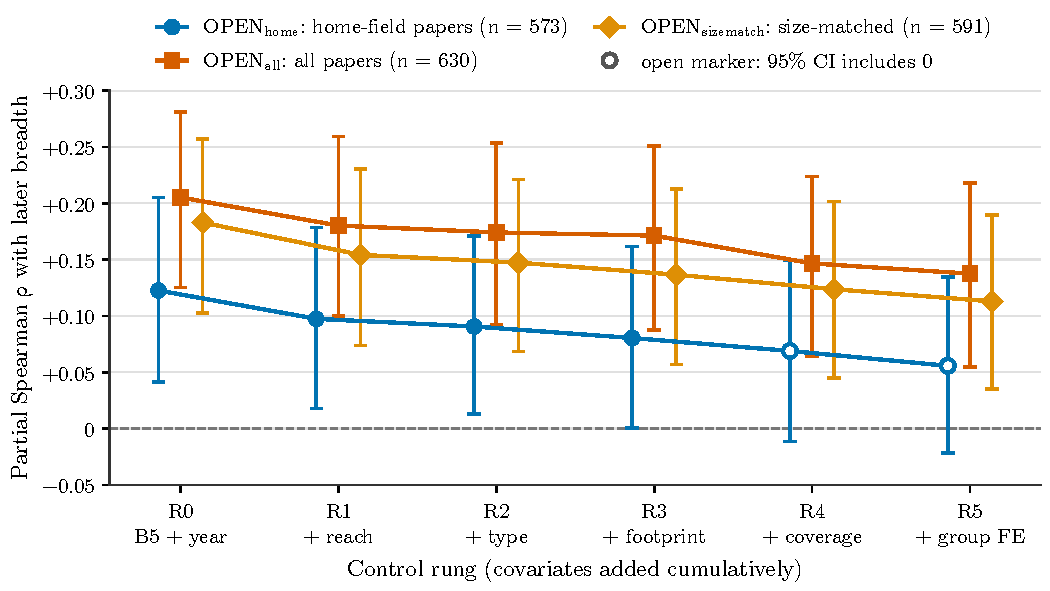
\includegraphics[width=\linewidth,height=0.85\textheight,keepaspectratio]{figures/fig_open_ladder_v0.pdf}
\caption{Control ladder for the OPEN index on the fresh 2015--2017 onset cohort. Circles are point estimates; error bars are 95\% CIs ($B = 2{,}000$). OPEN$_{\mathrm{home}}$ (blue) becomes marginal at R4/R5. OPEN$_{\mathrm{all}}$ (red) survives all rungs but is mechanically coupled.}
\label{fig:open_ladder}
\end{figure}

\subsection{Experiment~11: Does closing up at home slow a concept's spread? (incomplete)}

Sealed a within-concept pre-registration and ran DEV body models on 35{,}328 concept-years (4{,}661 concepts). Both pre-registered effects are null: density PPML $b = -0.070$ [$-0.180$, $+0.040$]; OPEN$_{\mathrm{home}}$ $b = +0.015$ [$-0.038$, $+0.069$]. By the frozen rule, this is NOT SUPPORTED. The Sun--Abraham event study was interrupted; held-out and cohort were not run. This is a dead end: the within-concept closure--entry mechanism was tested and was null on DEV.

\subsection{Experiment~12: How concepts spread -- contact versus keeping}

RQ2 trajectories analysis on all 12{,}499 Exp5 frame concepts, re-running the failed Exp9.

\paragraph{Breadth decomposition.} Log $B_n = \log E_2 + \log M + \log \rho$ (early contact diversity, frontier advance, retention). On 3{,}188 DEV concepts (variant i\_pooled):

\begin{table}[!htbp]
\centering
\caption{Breadth decomposition: share of the top-versus-bottom tercile gap in rarefied breadth attributable to each component (iteration~4, gen\_art\_experiment\_12).}
\label{tab:decomp}
\small
\begin{tabular}{lcc}
\toprule
Component & Share & 95\% CI \\
\midrule
Exploration ($s_{E2} + s_M$) & 0.732 & [0.703, 0.764] \\
\quad Early contact diversity ($s_{E2}$) & 0.779 & [0.738, 0.818] \\
\quad Frontier advance ($s_M$) & $-0.046$ & [$-0.074$, $-0.017$] \\
Retention ($s_\rho$) & 0.268 & [0.236, 0.297] \\
Difference (explore $-$ retain) & 0.464 & [0.407, 0.528] \\
\bottomrule
\end{tabular}
\end{table}

Note: these shares are an accounting identity for the breadth outcome (Bn and O2r share papers), not causal effects. The pre-registered PR1 test is variant iv (Medicine excluded): DEV 0.633 [0.537, 0.727], held-out pooled 0.492 [0.403, 0.575], cohort 0.445 [0.358, 0.527], DL 0.504 [0.329, 0.679], $I^2 = 0.76$. PR1 is SUPPORTED everywhere.

\begin{figure}[!htbp]
\centering
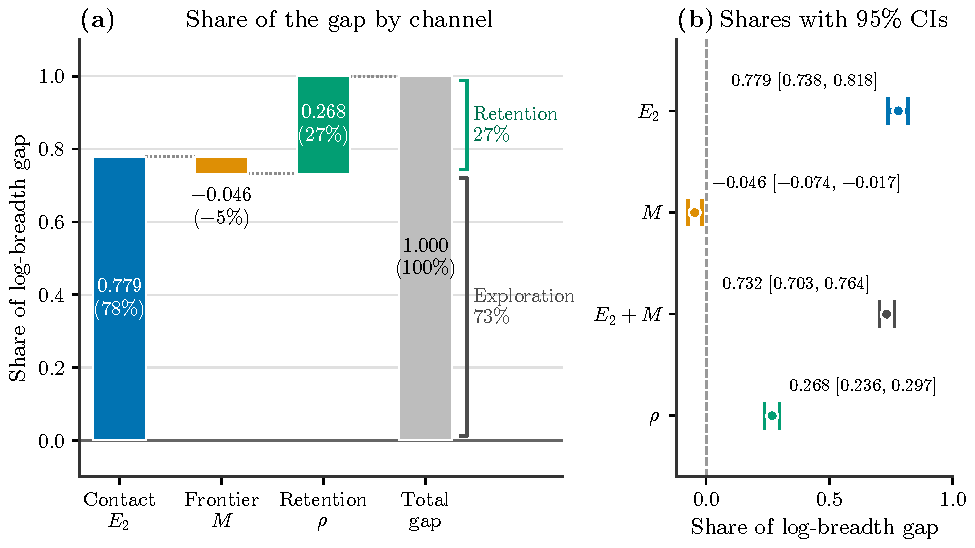
\includegraphics[width=\linewidth,height=0.85\textheight,keepaspectratio]{figures/fig_decomp_v0.pdf}
\caption{Log-additive decomposition of the gap in retained off-home breadth between the top and bottom terciles. Early contact diversity $E_2$ (blue) contributes 78\%, frontier advance $M$ (amber) is slightly negative, and retention $\rho$ (green) contributes 27\%.}
\label{fig:decomp}
\end{figure}

\paragraph{Typology.} No trajectory typology passes the naming rule: DTW $k = 4$ vs HMM $S = 5$ ARI $= 0.222$; held-out recluster ARI 0.44/0.38. Verdict: CONTINUUM. PC1 (38.8\%) is the breadth-of-spread axis; PC2 (10.7\%) is the keep-vs-lose axis.

\paragraph{OPEN and the trajectory axes.} OPEN correlates with PC1 (breadth) beyond B5: DEV partial 0.174/0.117/0.135 (ALL/HOME/SIZEMATCH); held-out DL 0.120/0.060/0.094 ($I^2 = 0$). OPEN does not correlate positively with the keeping axis (PC2 partial $-0.07$ to $-0.11$).

\paragraph{Sequence test.} No ordering signal beyond the mechanical lag (excess $\leq 1.7$ pp, sign flips). Intersection-born concepts take off later (HR $\approx 0.47$ [0.42, 0.54]).

\subsection{Evaluation~3: Record fixes and openness robustness tests}

\paragraph{Pre-onset footprint.} About half of the two biggest breadth effects is pre-onset footprint: M0\_\allowbreak density\_\allowbreak end drops from $+0.374$ to $+0.187$ post-onset (attenuation 0.50 [0.38, 0.60]); D\_\allowbreak vol\_\allowbreak end drops from $+0.317$ to $+0.176$ (0.45).

\paragraph{Specification curve.} 1{,}920 specifications (120 composites $\times$ 4 outcomes $\times$ 4 control sets): 99.7\% of pooled CIs above zero; median 0.152; Freedman--Lane $p = 0.005$. Note: this is exploratory, on the all-papers OPEN build, and uses groups already unsealed.

\paragraph{OPEN evidence pool (descriptive, on existing held-out data).} OPEN$_{\mathrm{home}}$ over 6 non-selection bodies: DL $+0.069$ [$+0.038$, $+0.100$], HKSJ [$+0.042$, $+0.096$], $I^2 = 0$, 6/6 positive. DEV selection body $+0.109$; shrinkage ratio 1.58.

\subsection{Research~3: Is `keep exploring, spread widest' already known?}

Claim C1 (openness $\to$ breadth): PARTIALLY ANTICIPATED. Maillart (2026) shows concept-pair diffusion with test $R^2$ 0.69/0.78; Wang (2017) shows foreign-field citation odds $+62\%$; Weng (2013) and Ugander (2012) show the effect for memes and people. No study found combines the concept unit, a size-adjusted breadth outcome, and held-out fields.

Claim C2 (consolidation $\to$ less breadth): PARTIALLY ANTICIPATED in mechanism, CONTRADICTED on other outcomes by Cheng et al.\ (2023) ($+53\%$ next-year volume per SD of ideational consistency).

\subsection{Iteration~4 dead ends}

\begin{enumerate}
\item Experiment~11 within-concept closure test: NOT SUPPORTED on DEV.
\item PR2 (``localised keep more early''): REVERSED on DEV ($-0.110$) and cohort ($-0.058$).
\item Two trajectory classes: CONTINUUM (DTW-HMM ARI 0.222).
\item Community-span indicators ($n_{\mathrm{comm}}$, participation) null in the home-only build.
\item OPEN$_{\mathrm{home}}$ predictive gain: negligible ($+0.002$).
\end{enumerate}

\subsection{Iteration~4 review and hypothesis update}

Review scored 2 (blocking), soundness~1 (fabricated case-study rows found; one executed artifact missing). The hypothesis sharpened from six-component ``openness'' to the decoupled home-only signal: novel partners (NOV$_{\mathrm{res}}$) and churn (edge persistence). The move was \textbf{deepen}: confirm on a vocabulary-free population (Frame~N) and test the Cheng reversal.


% ============================================================
\section{Iteration 5: Home-field churn on brand-new phrases}
\label{sec:iter5}

\subsection{Strategy and rationale}

Five artifacts were commissioned: (1) Experiment~13, Frame~N vocabulary-free confirmation; (2) Experiment~14, Cheng reach-vs-depth reversal; (3) Experiment~15, mechanism and Exp11 completion; (4) Evaluation~4, record repair and evidence pool; (5) Experiment~16, thin-sample confound check.

\subsection{Experiment~13: Does the churn signal hold for brand-new phrases?}

Mined 636 vocabulary-free phrase-born concepts from random title samples (2003--2015 onsets), excluding all legacy labels and previously scored concepts. These newborns have 14\% lower breadth and 89\% higher transience than legacy concepts, confirming vocabulary survivorship bias.

\paragraph{Result: PARTIAL.} OPEN$_{\mathrm{home}}$ PSP $= +0.117$ [$+0.020$, $+0.218$] at R3; $+0.086$ [$-0.009$, $+0.190$] at R5. On O2r$_{m50}$: $+0.161$ and $+0.122$, both CIs $> 0$. NOVCHURN$_{\mathrm{home}}$ at R3: $+0.108$ [$+0.007$, $+0.211$]. DL $+0.112$ [$-0.015$, $+0.239$]; Holm $p = 0.052$.

\paragraph{Components.} NOV$_{\mathrm{res}}$ carries the signal ($+0.208$ [$+0.113$, $+0.303$]); edge persistence is null ($-0.013$).

\paragraph{Cheng reversal not confirmed on Frame~N.} PSP $-0.064$ [$-0.159$, 0.031].

\paragraph{Exploratory pool.} Pooling Frame~N with the legacy cohort (Exp10) at R3 gives $+0.096$ [$+0.034$, $+0.158$].

\begin{figure}[!htbp]
\centering
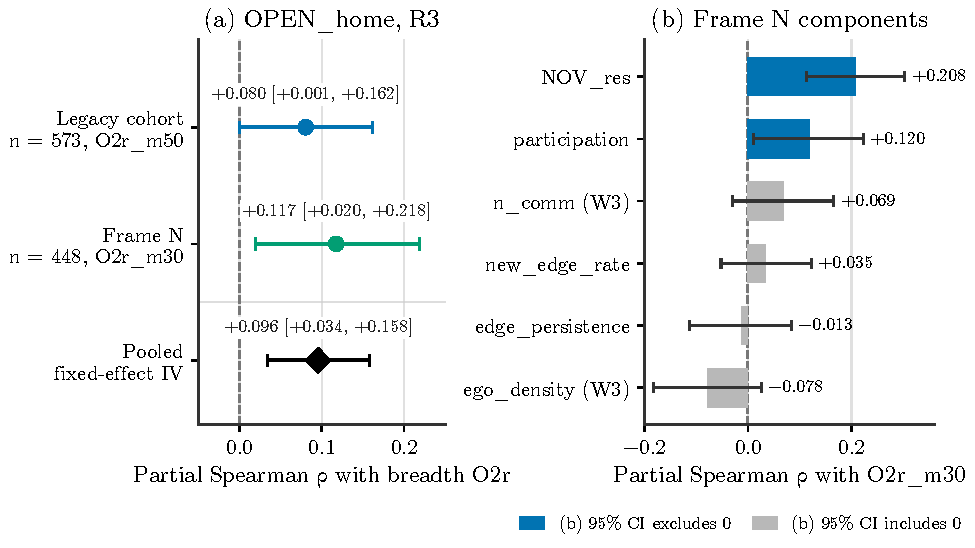
\includegraphics[width=\linewidth,height=0.85\textheight,keepaspectratio]{figures/fig_frame_n_v0.pdf}
\caption{Confirmation of the OPEN signal on vocabulary-free Frame~N concepts. (a) OPEN$_{\mathrm{home}}$ PSP at R3: legacy cohort $+0.080$, Frame~N $+0.117$, exploratory pool $+0.096$. (b) Component PSPs on Frame~N: NOV$_{\mathrm{res}}$ carries the signal ($+0.208$); edge persistence is null.}
\label{fig:frame_n}
\end{figure}

\subsection{Experiment~14: Cheng's consistency is a size effect, not a reach predictor}

Rebuilt Cheng et al.'s (2023) ideational consistency measure on 12{,}311 concepts (105{,}839 concept-years).

\paragraph{Test A: Cheng design reproduced.} NB twin: $b = 0.428$ ($+53.5\%$/SD). Adding current volume $\log V(t)$: $+1.3\%$ [$+0.5\%$, $+2.1\%$]; ratio A2/A1 $= 0.021$ [0.009, 0.035]. The volume effect is almost entirely a proxy for current size.

\paragraph{Test B: Consistency predicts \emph{narrower} breadth.} PSP with O2r$_{m50}$ given B5: $-0.069$ [$-0.093$, $-0.047$]; DL over 5 groups $-0.079$, $I^2 = 0$, 5/5 negative. Replicated on 2015--2017 cohort: $-0.111$ [$-0.197$, $-0.030$].

\paragraph{Test C: Within-concept.} Consistent years followed by slightly \emph{more} off-home entries ($b = +0.025$, CI [0.004, 0.048]); the reach penalty is a between-concept trait.

\paragraph{Test D.} No Palla size $\times$ consistency interaction.

\paragraph{Identity.} Spearman 0.77 with Jaccard edge persistence.

\begin{figure}[!htbp]
\centering
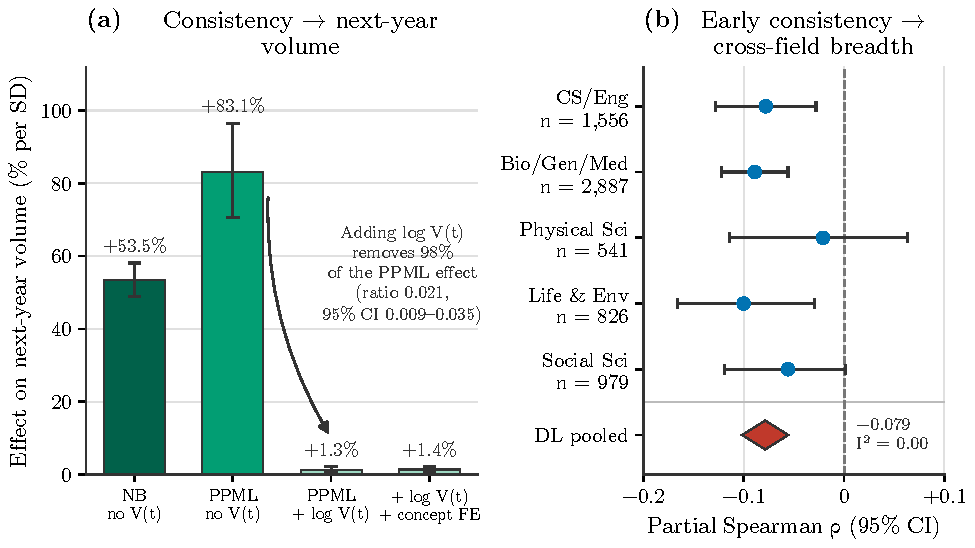
\includegraphics[width=\linewidth,height=0.85\textheight,keepaspectratio]{figures/fig_cheng_reversal_v0.pdf}
\caption{The consistency--breadth reversal. (a) Consistency predicts next-year volume: $+53.5\%$ without $V(t)$; $+1.3\%$ with $V(t)$ (98\% removed). (b) Consistency predicts \emph{narrower} breadth: DL pooled $-0.079$ [$-0.102$, $-0.056$], $I^2 = 0$, 5/5 groups negative.}
\label{fig:cheng_reversal}
\end{figure}

\subsection{Experiment~15: Why churning concepts spread; Exp11 completion}

Three parts.

\paragraph{Part C: Exp11 completion.} DEV verdict unchanged: NOT SUPPORTED. Old held-out: OPEN$_{\mathrm{home}}$ $-0.079$ [$-0.146$, $-0.013$], the opposite of the predicted sign. Sun--Abraham event study (DEV never-treated): lag 0..2 $= -0.018$ [$-0.042$, $+0.004$], pre-trend $p = 0.52$. H-S1 (home-to-off-home) holds on DEV ($+0.113$), cohort ($+0.105$) and pooled ($+0.076$ [$+0.024$, $+0.126$]) but not on old held-out ($+0.001$). H-P1 fails as pre-registered.

\paragraph{Part A: Partner decomposition.} NOVCHURN$_{\mathrm{home}}$ pooled: $+0.118$; held-out DL $+0.097$ ($I^2 = 0$). The signal comes from:
\begin{itemize}
\item New-community partners ($C_2 = +0.102$ [$+0.069$, $+0.133$], Holm $p = 0.0025$).
\item Partners from mixed-field papers ($C_4 = +0.103$ [$+0.071$, $+0.134$], Holm $p = 0.0025$).
\item Domain partners, not methodological partners (domain Shapley $\phi = +0.132$ on the 2015--2017 cohort; method $= +0.012$).
\end{itemize}
Bridging papers (5\% of early home papers) halve NOVCHURN's PSP from 0.118 to 0.056.

\paragraph{Part B: Trait stability.} Yearly OPEN$_{\mathrm{home}}$ ICC: 0.37/0.34/0.39. Window retest: 0.51--0.57. Prediction P-B1 FAILS.

\begin{figure}[!htbp]
\centering
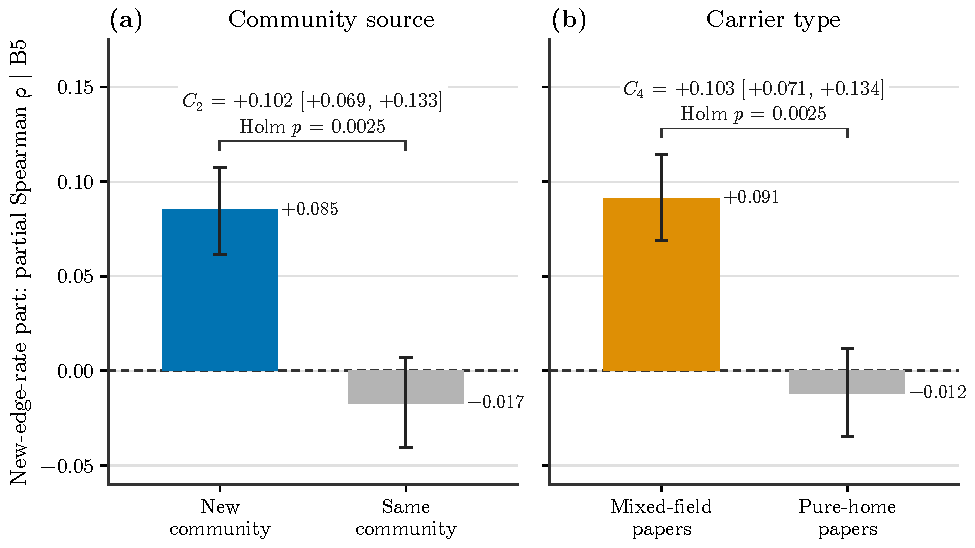
\includegraphics[width=\linewidth,height=0.85\textheight,keepaspectratio]{figures/fig_mechanism_v0.pdf}
\caption{Which co-occurrence partners carry the signal? (a) New-community partners (blue, $+0.085$) carry it; same-community (grey, $-0.017$) do not. (b) Mixed-field paper partners (orange, $+0.091$) carry it; pure-home (grey, $-0.012$) do not.}
\label{fig:mechanism}
\end{figure}

\subsection{Experiment~16: Is neighbourhood churn real or thin-sample noise?}

Confound check on 13{,}444 selection concepts with $n_{\mathrm{home,early}} \geq 10$.

\paragraph{Mechanical verdict: PARTLY THIN.} Raw persistence has Spearman $+0.72$ with log home-paper count. The within-concept year-permutation null absorbs the temporal component: excess NOVCHURN PSP $= +0.008$ [$-0.02$, $+0.03$] (raw: $+0.116$). The $R^2$ of raw persistence on the permutation-null mean is 0.66. The signal is a static topical-dispersion property of the home topic mix, not year-to-year turnover. V2 excess variants have split-half $r_{SB}$ of $\sim$0.01--0.05 and the planted-churn check (PC2) fails, so V2 cannot adjudicate temporal churn at $\sim$10 papers/year.

\paragraph{Corrections that help.} Fixed-$n$ rarefaction ($n = 10$) retains 68\% of the pooled association. Degree-preserving configuration $z$-score raises OPEN$_{\mathrm{home}}$ from $+0.092$ to $+0.115$ on the same sample ($+0.022$ [0.011, 0.034]).

\paragraph{Reliability.} Split-half $r_{SB}$: NOVCHURN$_{\mathrm{raw}}$ 0.48, OPEN$_{\mathrm{home}}$ 0.49, OPEN$_{\mathrm{home,clean}}$ 0.58, outcome O2r$_{m50}$ 0.895. Disattenuated pooled NOVCHURN$_{\mathrm{raw}}$ PSP: 0.178 [0.141, 0.214] (approximate).

\begin{figure}[!htbp]
\centering
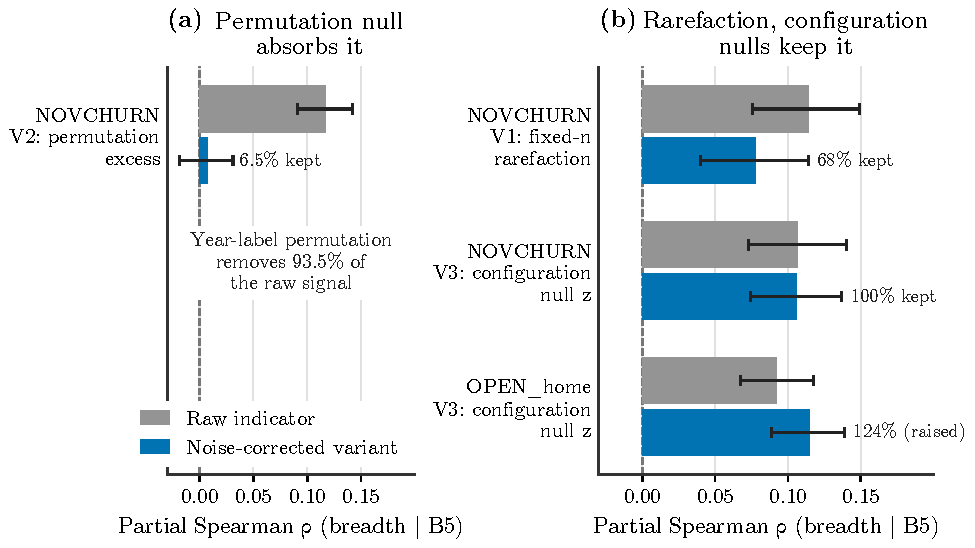
\includegraphics[width=\linewidth,height=0.85\textheight,keepaspectratio]{figures/fig_confound_v0.pdf}
\caption{The churn/openness signal behaves like topical non-redundancy, not temporal turnover. (a) The within-concept permutation excess cuts NOVCHURN from $+0.117$ to $+0.008$, keeping 6.5\%. (b) Fixed-$n$ rarefaction keeps 68\%; configuration-null $z$-score raises OPEN$_{\mathrm{home}}$ to 124\%.}
\label{fig:confound}
\end{figure}

\subsection{Evaluation~4: Record repair and openness evidence pool}

\paragraph{Evidence synthesis (descriptive).} OPEN$_{\mathrm{home}}$ non-selection pool ($k = 6$: 4 held-out groups + 2 cohort parts): DL $+0.069$ [$+0.038$, $+0.100$], HKSJ [$+0.042$, $+0.096$], $I^2 = 0$, 6/6 positive. DEV selection body $+0.109$; shrinkage ratio 1.58. NOVCHURN$_{\mathrm{home}}$ ($k = 5$): DL $+0.105$ [$+0.069$, $+0.140$].

\paragraph{Claims ledger.} v4: 1{,}769 rows, 0 MISMATCH, 0 NOT\_FOUND, 0 orphans.

\subsection{Iteration~5 dead ends}

\begin{enumerate}
\item Frame~N Cheng reversal: not confirmed (PSP $-0.064$, CI includes 0).
\item Edge persistence on Frame~N: null ($-0.013$).
\item Temporal turnover as mechanism: V2 excess unreliable (split-half 0.01--0.05).
\item Trait prediction (P-B1): fails (ICC 0.34--0.39).
\item METHOD partner excess: DEV-only, not replicated in cohort.
\item Within-concept closure (Exp11): NOT SUPPORTED on DEV; opposite-signed on held-out.
\end{enumerate}

\subsection{Iteration~5 review and hypothesis update}

Review scored 2 (blocking). Confidence decreased further. The headline surviving signal is: concepts whose home-field co-occurrence partners span many communities and arrive through mixed-field papers tend to reach more fields later. The effect size is modest (OPEN$_{\mathrm{home}}$ non-selection pool $+0.069$, $I^2 = 0$), adds no practical forecasting gain, and the temporal interpretation is untested rather than confirmed.


% ============================================================
\section{What the run learned overall}
\label{sec:lessons}

\subsection{Confirmed findings}

\begin{enumerate}
\item \textbf{Indicator screen.} Seven of 53 early co-occurrence network indicators survive held-out validation for predicting rarefied cross-field breadth, spanning two families (retained frontier and co-occurrence topology). The strongest purely post-onset indicators are CONTACT\_REACH ($+0.211$), $n_{\mathrm{comm}}$ ($+0.167$) and NOV$_{\mathrm{res}}$ ($+0.151$).

\item \textbf{OPEN index.} The Eval4 descriptive pool of OPEN$_{\mathrm{home}}$ over 6 non-selection bodies gives partial Spearman $+0.069$ [$+0.038$, $+0.100$], $I^2 = 0$, 6/6 positive. Evidence state: lead. On the fresh cohort, OPEN$_{\mathrm{home}}$ is $+0.091$ at R2 but marginal at R4/R5 (DL includes 0). No forecasting gain over B5.

\item \textbf{Consistency--breadth reversal.} Cheng et al.'s (2023) ideational consistency predicts next-year volume ($+53\%$/SD) but \emph{narrower} breadth (PSP $-0.069$, $I^2 = 0$, 5/5 groups negative). Adding current volume removes 98\% of the volume effect.

\item \textbf{Retained-field relatedness.} Concepts spread next to fields related to those currently retaining them ($d_0 = 0.322$ [0.291, 0.355] on the independent frame). Verdict: FRONTIER = PARTIAL (volume-matched contrast null; reverses under min-cp proximity).

\item \textbf{Breadth decomposition.} Early contact diversity accounts for $\sim$73\% of the breadth gap; frontier advance contributes near zero. This is an accounting identity, not a causal decomposition.

\item \textbf{Background homophily.} 100\% of 48 concepts have positive background log-odds ratios; $R^2 = 0.66$. Raw lineage metrics are mostly field composition, not concept-specific integration.
\end{enumerate}

\subsection{What failed and why}

\begin{enumerate}
\item \textbf{Naturalisation gap $A^*_h$}: null ($\Delta\rho = -0.006$), 0/4 groups, low reliability.
\item \textbf{Gateway-field retention}: disconfirmed at scale ($\Delta$AUC $-0.00001$); it was a domain-specific proxy.
\item \textbf{Gateway landing $G$}: small, pooled CI includes zero, a quarter of DEV value.
\item \textbf{Co-occurrence diversity $D$, selectivity $F$}: null on the DEV panel.
\item \textbf{Rescue, relay, ordering}: not supported or MIXED.
\item \textbf{Two trajectory classes}: not reproduced by HMM (ARI 0.094); CONTINUUM.
\item \textbf{Within-concept closure}: NOT SUPPORTED (Exp11 null on DEV, opposite-signed on held-out).
\item \textbf{External recognition O5}: unrelated to breadth ($\rho = 0.014$); 67\% recognised before onset.
\item \textbf{Candidate S (co-author groups)}: tested in Exp8, not confirmed for any outcome.
\item \textbf{RETENTION\_RATIO\_early}: attenuates on the fresh cohort; does not survive concept-type controls.
\end{enumerate}

\subsection{What is still open}

\begin{enumerate}
\item Temporal turnover vs static dispersion: the V2 excess is unreliable at typical sample sizes, so whether the signal is truly temporal could not be adjudicated.
\item Domain heterogeneity: Life \& Environment shows the weakest OPEN signal (PSP $+0.071$ vs $+0.186$ for other units pooled). The reason is unexplained.
\item Causal mechanism: early ego-network openness could reflect the concept's intrinsic generality, the diversity of the research community, or the breadth of the problems addressed. Only association is shown.
\item The persistence-filtered RCA density rival ($D_{\mathrm{rca,persist,k}}$) differs from Exp7's $D_{\mathrm{rca,pers}}$ (max $\rho = 0.877$) and remains formally untested.
\item No discrete trajectory typology passes the naming rule; whether there are real types beyond the continuum is unresolved.
\end{enumerate}


% ============================================================
\section*{Appendix: Artifact inventory}
\label{sec:inventory}

\begin{longtable}{p{1.5cm}p{4.5cm}p{2cm}p{4.5cm}}
\caption{All artifacts commissioned across five iterations.} \label{tab:inventory} \\
\toprule
Iter. & Artifact & Status & Key result \\
\midrule
\endfirsthead
\toprule
Iter. & Artifact & Status & Key result \\
\midrule
\endhead
\bottomrule
\endfoot
1 & gen\_art\_experiment\_1 & Completed & $A^*_h$ null ($\Delta\rho = -0.006$) \\
1 & gen\_art\_experiment\_2 & Failed & Candidate S untested (stalled) \\
1 & gen\_art\_experiment\_3 & Completed & $D$/$F$ null; portability table \\
1 & gen\_art\_experiment\_4 & Completed & $G$ null; retention lead +0.103 \\
1 & gen\_art\_dataset\_1 & Failed & Held-out frame not built (stalled) \\
\midrule
2 & gen\_art\_experiment\_5 & Completed & H1 disconfirmed; 12{,}499-concept frame \\
2 & gen\_art\_experiment\_6 & Completed & H2 $d_0 = 0.302$; trajectories \\
2 & gen\_art\_evaluation\_1 & Completed & Gateway fails stress test \\
2 & gen\_art\_dataset\_2 & Completed & O5 recognition table \\
2 & gen\_art\_research\_1 & Completed & ANS positioning \\
\midrule
3 & gen\_art\_experiment\_7 & Completed & FRONTIER = PARTIAL ($d_0 = 0.322$) \\
3 & gen\_art\_experiment\_8 & Completed & 7/10 indicators confirmed \\
3 & gen\_art\_experiment\_9 & Failed & RQ2 trajectories (format error) \\
3 & gen\_art\_evaluation\_2 & Completed & 246-claim audit \\
3 & gen\_art\_research\_2 & Completed & Prior art verdicts \\
\midrule
4 & gen\_art\_experiment\_10 & Completed & OPEN$_{\mathrm{home}}$ +0.091 (marginal) \\
4 & gen\_art\_experiment\_11 & Incomplete & Closure test null on DEV \\
4 & gen\_art\_experiment\_12 & Completed & Decomposition; CONTINUUM \\
4 & gen\_art\_evaluation\_3 & Completed & Footprint rescore; spec curve \\
4 & gen\_art\_research\_3 & Completed & Novelty verdicts \\
\midrule
5 & gen\_art\_experiment\_13 & Completed & Frame~N PARTIAL (+0.117) \\
5 & gen\_art\_experiment\_14 & Completed & Cheng reversal confirmed \\
5 & gen\_art\_experiment\_15 & Completed & Partner decomposition; Exp11 done \\
5 & gen\_art\_evaluation\_4 & Completed & Evidence pool +0.069 \\
5 & gen\_art\_experiment\_16 & Completed & PARTLY THIN; static dispersion \\
\end{longtable}

\end{document}
